\onehalfspacing

\section{Neutrino Research}

\noindent Neutrinos are the most abundant non-massless particle \cite{Vitagliano}, yet due to their nature very little is known about them. Neutrinos are charge neutral particles and only interact through the weak interaction (and the force of gravity), meaning detecting them can is extremely difficult \cite{Maki}. Every second, a large number of neutrinos pass through the earth and through people in the form of solar neutrinos and high energy cosmic rays \cite{Szadowski}. \medskip

\noindent To isolate the detectors from other background radiation many experiments and detectors are placed deep underground. Many cosmic neutrinos penetrate through the ground and to the detectors, however they are able to be accounted for and excluded from the analysis. There are a number of underground neutrino experiments, notably MINER$\nu$A \cite{Perdue}, IceCube, \cite{Brenzke}, Super-Kamiokande \cite{Fukuda_1} and Dune \cite{Acciarri_1}, however the experiment that this project is working on is the NOvA experiment at Fermilab \cite{Aurisano}. \medskip

\noindent It was observed that two thirds of atmospheric neutrinos that were expected to reach earth, which led to the observation that neutrinos have a mass and the ability to oscillate between the different flavours \cite{Fukuda_2}. This explained how the neutrinos expected to be observed changed to a different flavour, a discovery that was awarded the 2015 Nobel prize, however, the exact masses of the the flavours as well as the precise values of the oscillation parameters are still unknown \cite{Capozzi}. The three neutrino flavours, each named due to the associated lepton that is produced or absorbed with the neutrino, do not correlate to the mass eigenstates, but are a superposition of them, where $\ket{\nu_\alpha}$ is a neutrino with flavour $\alpha$ = $e$, $\mu$, $\tau$ for electron, muon and tau, and $\ket{\nu_i}$  a neutrino with definite mass $m_i$ for $i =1,2,3$, where $U$ is the PMNS matrix \cite{Giganti}. \medskip

 \[\ket{\nu_\alpha} = \sum_{i}U^ {*}_\alpha i  \ket{\nu_i}\]

\noindent Neutrinos interact with other particles in their flavour eigenstates, but travel as mass eigenstates. As a neutrino travels, the quantum mechanical phases of the mass eigenstates advance at different rates due to mass differences, which results in a changing superposition of mass eigenstates corresponding to a different flavour. This violated the Standard Model which predicted neutrinos as massless, requiring exploration beyond the Standard Model which could produce new unknown properties of fundamental particles \cite{Sonneveld}. \medskip


\section{NOvA Experiment}

\noindent To measure these oscillations, neutrino energy and flavours need to be reconstructed; as neutrinos are invariant to charge and magnetic fields they travel without deflection they indicate their sources of production, this means they can easily be traced back to an inception vertex, examples of these images are shown in Figure 1. If the flavour can be determined, which is the case for charged-current interactions (CC) from the associated lepton that is produced. The two charged current neutrino variants that are observed are $\nu_\mu$ and  $\nu_e$ events, as the lifetime of the  $\nu_\tau$ is short, and not visible to the detector \cite{Aurisano}.\medskip

\noindent The dominant CC interactions are: quasi-elastic - where the nucleon recoils from the scattering lepton; resonant - where the nucleon is deflected into baryonic resonance; deep-inelastic-scattering - where the nucleon breaks up in the process of hadronisation, and meson exchange currents - where two-nucleon emission takes place \cite{Aurisano}.\medskip

\noindent Neutral-current (NC) interactions don’t indicate an associated lepton, as they are observed though the interacting hadron, with the outgoing lepton being a neutrino - which goes on undetected- thus their flavour cannot be determined. \medskip

\begin{figure}
\centering
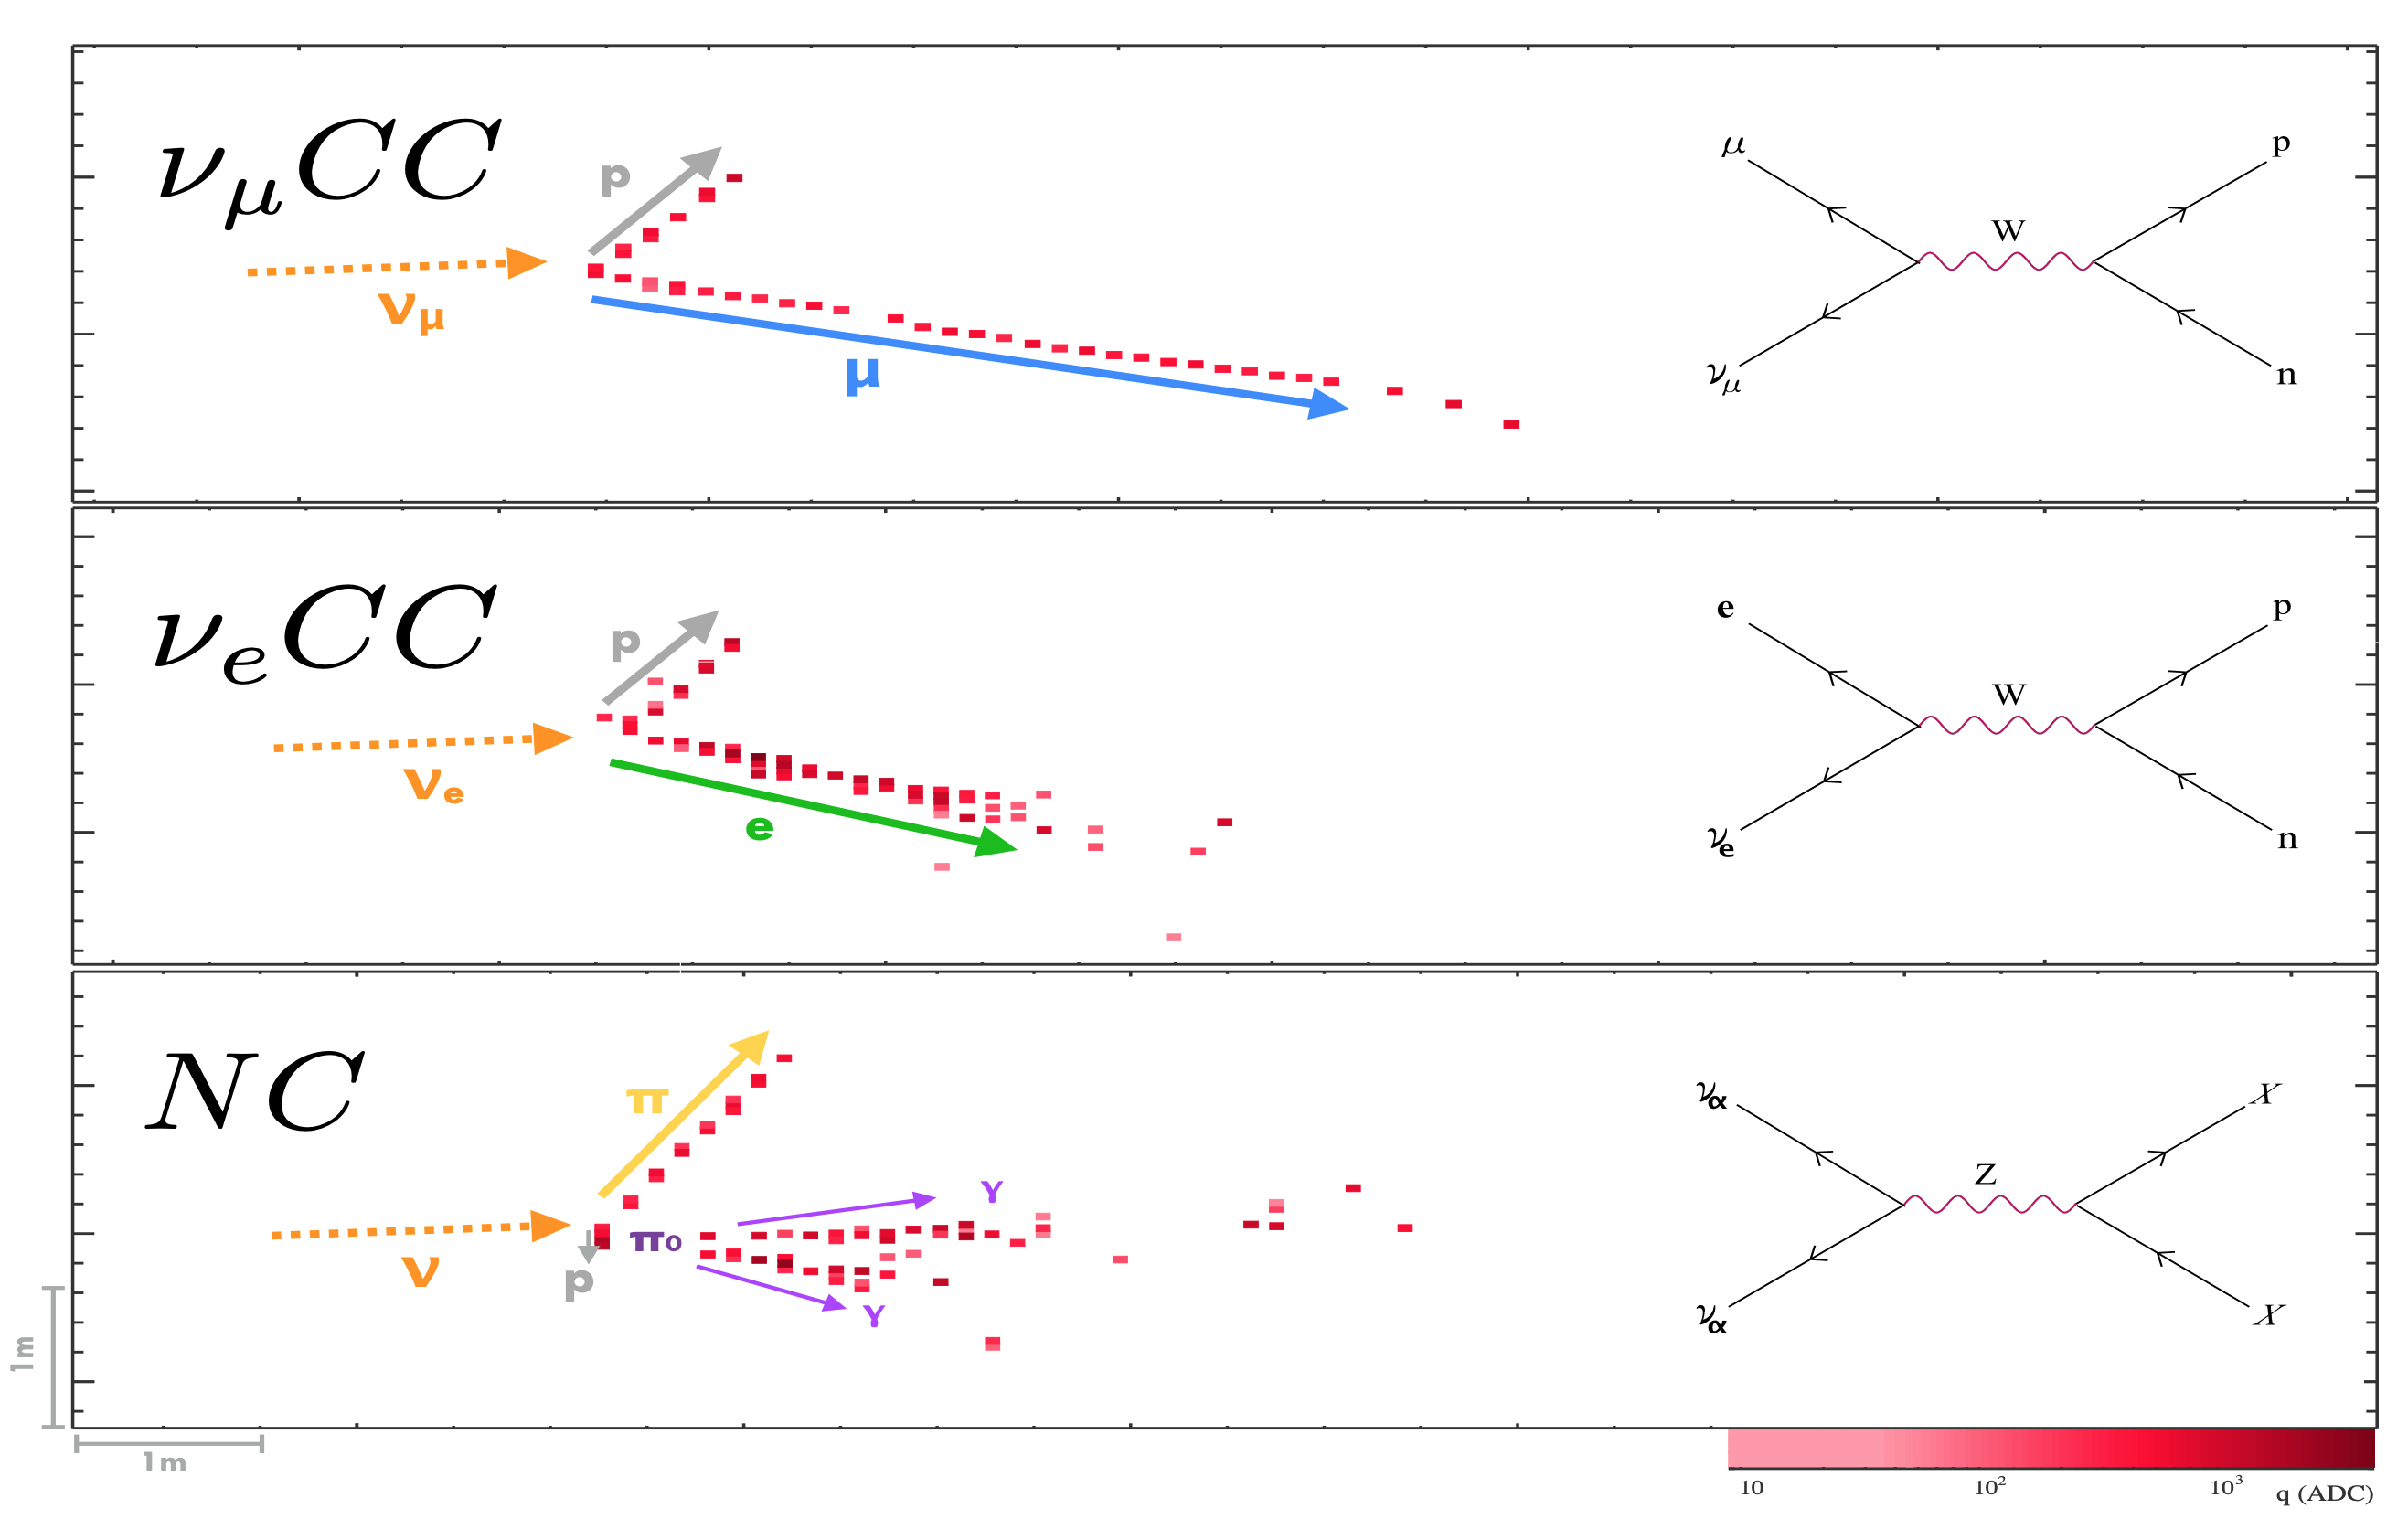
\includegraphics[scale=0.25]{Images/tracks.png}

 \textbf{Figure 1.} \textit{Three of the event topologies, for charged-current muon and electron neutrinos as well as a charged-neutral interaction, with their associated Feynman diagrams \cite{Singh}.}
\end{figure}

\noindent At NOvA a near detector, placed 1 km from the beam source, and a far detector, 810 km away, are used to determine the flavour of neutrino passing at each, and any changes to the neutrinos over the distance can be compared. By comparing the number of neutrinos of each flavour at the detectors, oscillation calculations can be made. \medskip

\noindent The detectors are a pair of finely grained liquid scintillator detectors. The near detector is 4m x 4m x 15m in size, with cells filled with liquid scintillator. Fibre optic cables collect the scintillation light to be stored. \medskip

\noindent The scintilator cells are arranged into planes, which are configured into horizontal and vertical alignments to provide separate, interleaved X-Z, and Y-Z views. The data therefore is displayed as the top view and side view of the detector, and these are what are used as inputs to the classification algorithm, see Figure 2 for a schematic of the detector and the output views.\medskip

\noindent A NuMI (Neutrinos at the Main Injector) beam, made of muon neutrinos is produced by firing protons into a graphine target, which produces pions amongst other particles. These pions are able to be directed by magnets in an intended direction of travel , before the pions decay into Muons and muon neutrinos. \cite{Ishitsuka} \medskip

\begin{figure}[t]
 \centering
 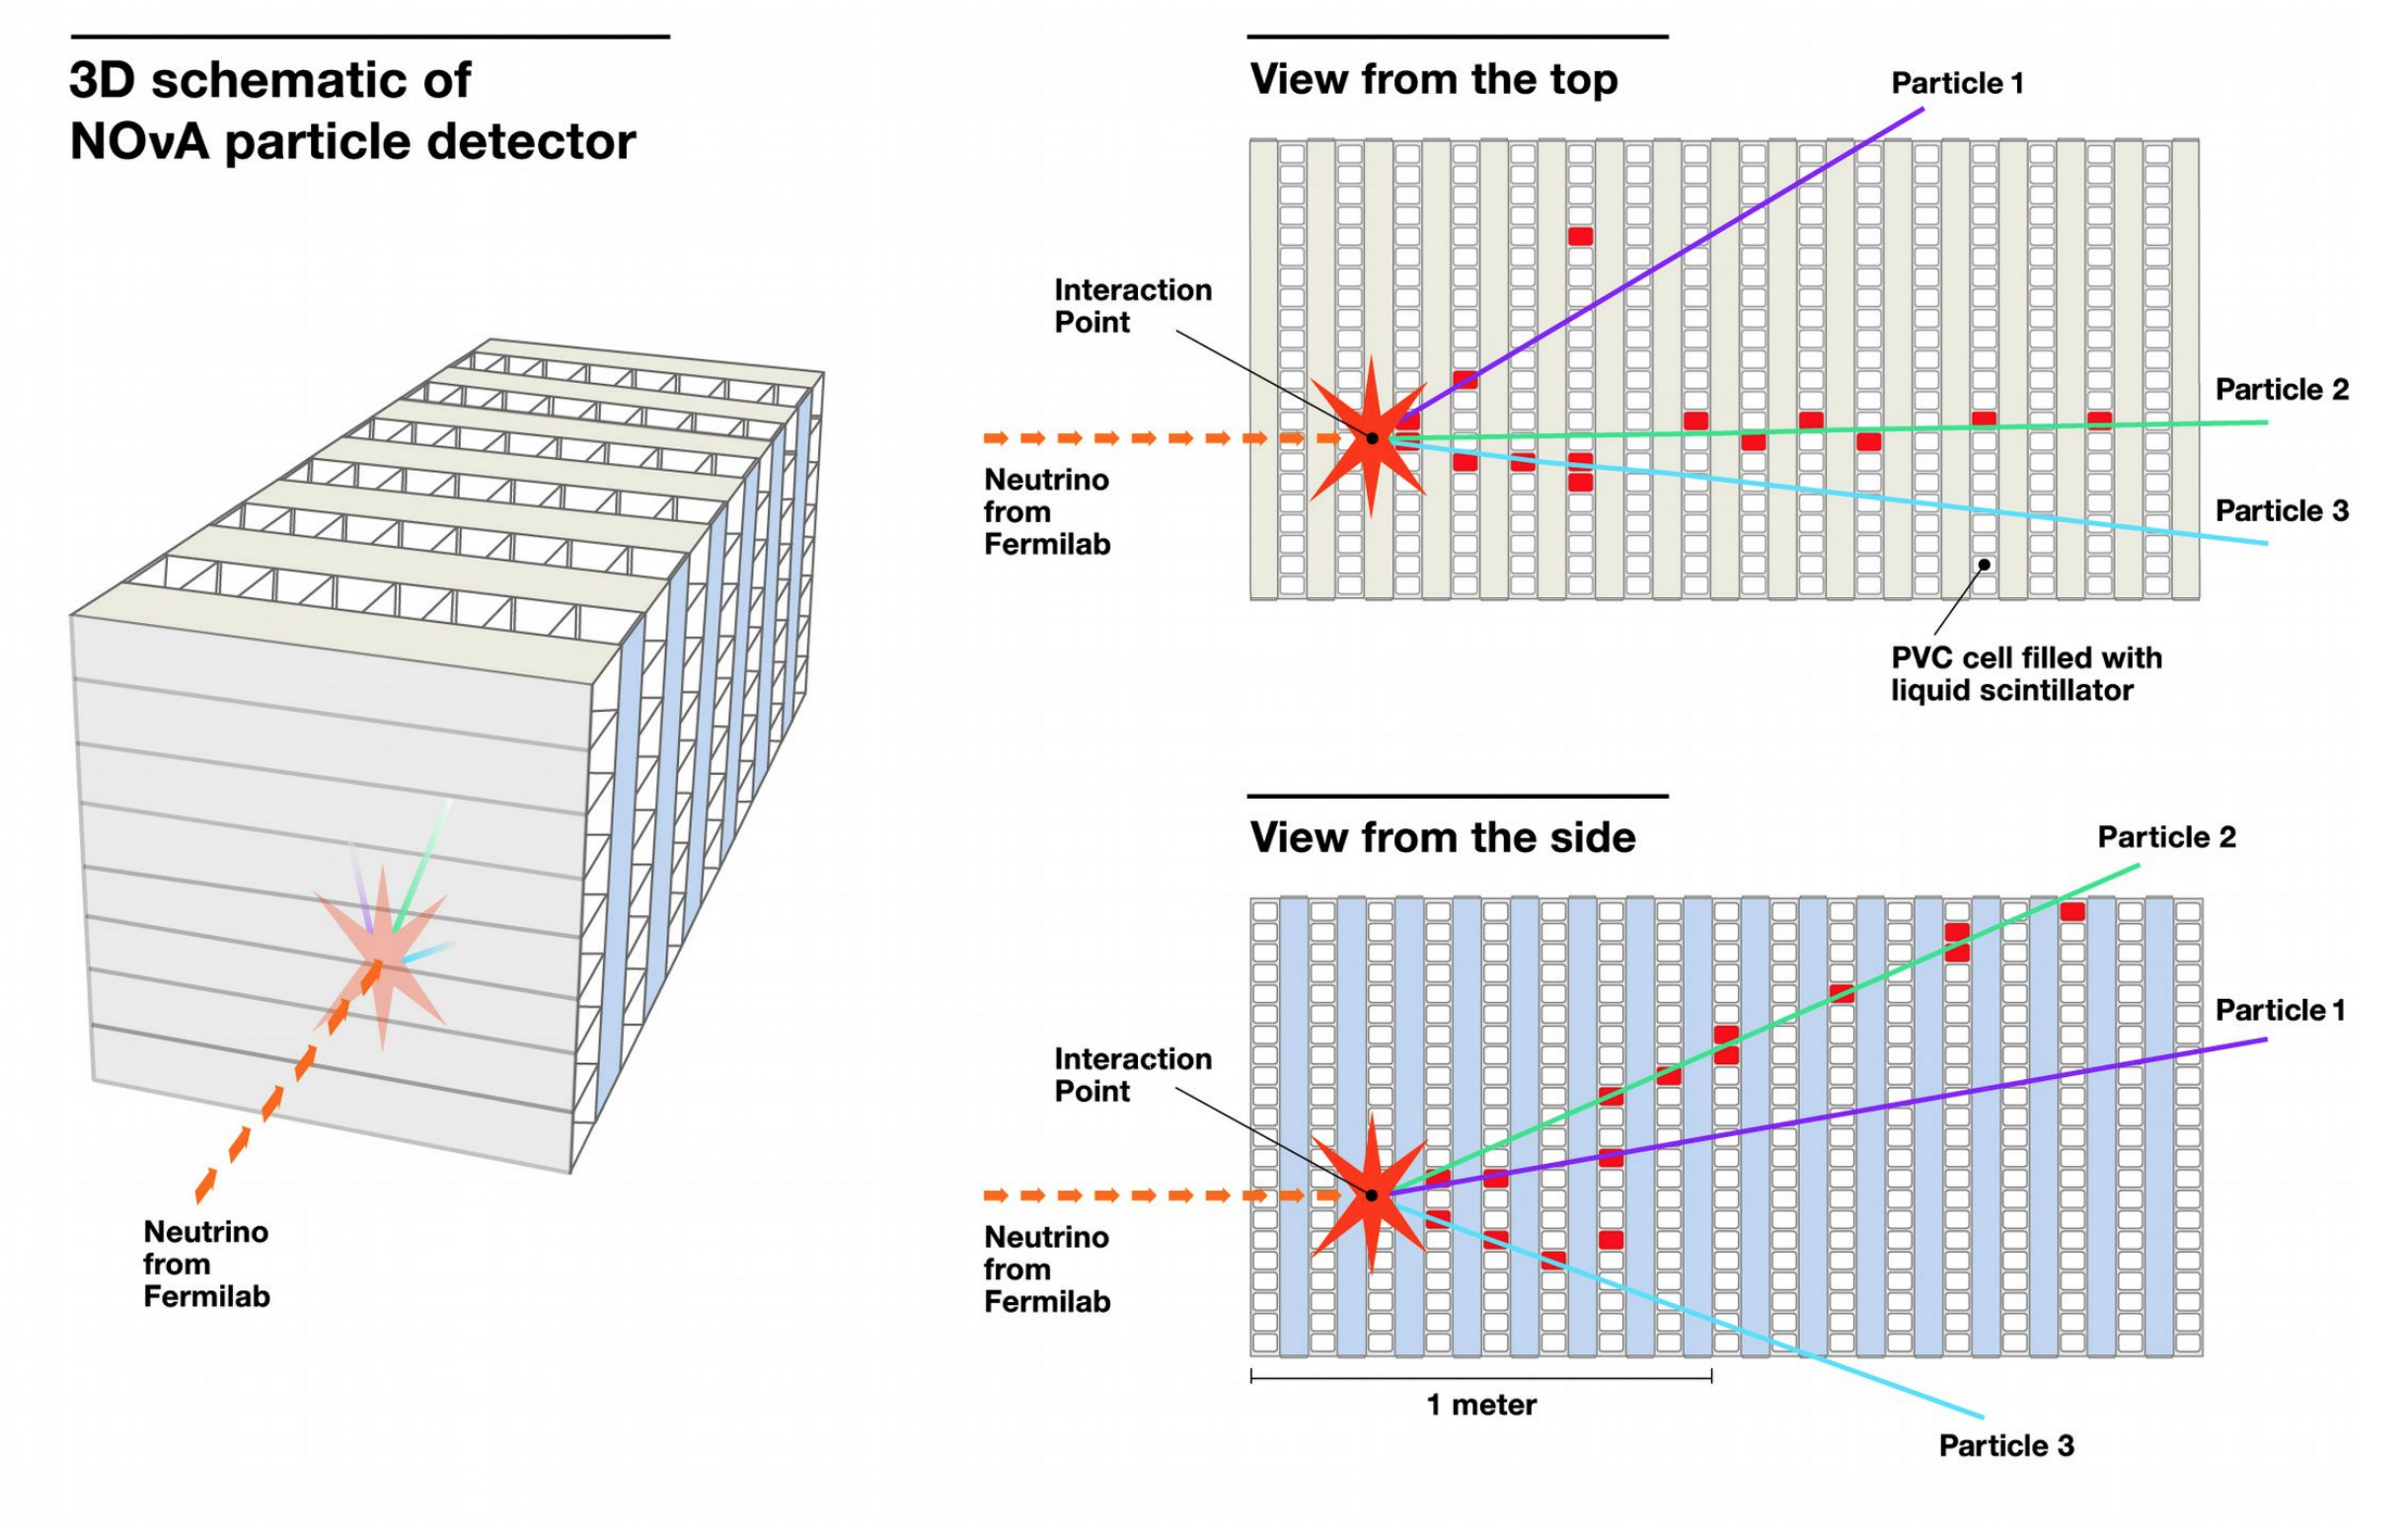
\includegraphics[scale=0.25]{Images/nova_nd.png} 
 
\textbf{ Figure 2.} \textit{Schematic of the NO$\nu$A scintilator detectors. The diagram on the left shows the 3D representation of the detector, while the diagrams on the right show the top view and side view planes where cell activation in each row or column indicate the tracks of the particles \cite{Aurisano}}.
\end{figure}

\noindent Traditionally classification required reconstructing high-level components associated with particle interactions such as clusters, tracks, showers, jets, and rings and summing the directions, and shapes of these objects, \cite{Aurisano}. However, the method now implemented at NOvA is a machine learning algorithm, where the model learns how to classify the interaction type from examples, a process known as supervised learning. Currently a CNN is being used, which has been found to be capable of pattern detection and particularly effective at image classification with real world photographs. \medskip

\noindent The network will look to classify the events based on features from the event topologies. $\nu_\mu$ events are indicated by a long, low dE/dx (energy loss per unit distance) track which is that of a minimally ionizing $\mu$, while $\nu_e$ events display a shower rather than a track . NC events can display both $\nu_\mu$ and  $\nu_e$ interaction like features- if the interaction produces pions. A charged pion track appears similar to that of a muon, except for an energy deposition spike at the end of the tracks; while the lifetime of a neutral pion is short, and it decays to produce electromagnetic shower, with the gap between the event vertex and shower the distinguishing factor from a $\nu_e$ event \cite{Aurisano}. \medskip

\noindent These similarities make the challenge of classification difficult, even for state of the art computer vision networks, however the performance compared to traditional reconstruction analysis showed positive results for these methods. NOvA's classifier, which at the time, was based on the GoogLeNet algorithm, that achieved an error rate of only 6.7\% on images \cite{Szegedy}, it now also uses the MobileNet algorthym that we will be using in this study, however they are yet to publish results of its performance. The network at NOvA outperforms the previous track-based modestly with a measurement-optimised efficiency of 58\% over the of 57\% from \cite{Adamson_1} for $\nu_\mu$ CC interactions and for $\nu_e$ CC interactions 49\% over the 35\% when compared to results from \cite{Adamson_2}. \medskip

\noindent In order to both learn how to classify as well as to validate the predictions against the actual classifications, the algorithms require labeled classification data as well as the event images. Data from the detector will not be labeled, thus simulated Monte Carlo event generators will provide the training examples; the two simulators that will be used are GENIE \cite{Andreopoulos_1} and GiBUU \cite{Lalakulich} however there are many different models that all simulate events uniquely. The GENIE Monte Carlo Simulation simulations the initial iteration of a neutrino with nuclei in the detector and the resulting scattered products to the surface of the nucleus \cite{Andreopoulos_2}. It mainly reproduces neutrino-nucleon scattering data but limited neutrino-nucleus scattering data means there are deficiencies in the primary physics model \cite{Perdue}. While the GiBUU simulation based on the Giessen–Boltzmann–Uehling– Uhlenbeck model which is a semiclassical transport model which describes the evolution of a many-body system in the presence of potentials and a collision term, with the addition  of neutrino-induced interactions. \medskip

\section{Machine Learning}

\noindent Artificial Neural networks (ANNs) \cite{McCulloch} are not a new phenomenon, however the recent increase in their popularity has come about due to the advances in hardware that allows the computationally expensive training of networks, which led to improvements in architectures and training processes. Neural networks increase in performance when given more data to learn from, and the volumes of data that are produced in this digital age has led to increased research into the development of theses algorithms. \medskip

\noindent In a traditional Feed Forward  Neural Network (FFNN), the most basic ANN, each neuron in each layer the output will be a weighted sum of the inputs from every neutron in the preceding layer, with this sum being passed to an activation function, which brings non-linearity allowing the modelling of more complex patterns \cite{Acciarri_2}. The output, $y_k$, for the $k^{th}$ neuron in a layer where $i = 1, 2,..., n$ where $n$ is the number of neutrons in the previous layer, and $x_{i}$ their corresponding outputs, with $w$, the weights, $b$, the bias, and $\sigma$ the activation function. \medskip

\[y_k = \sigma(\sum_{i}w_{ki} x_i +b)\]

\begin{figure}[t]
 \centering
 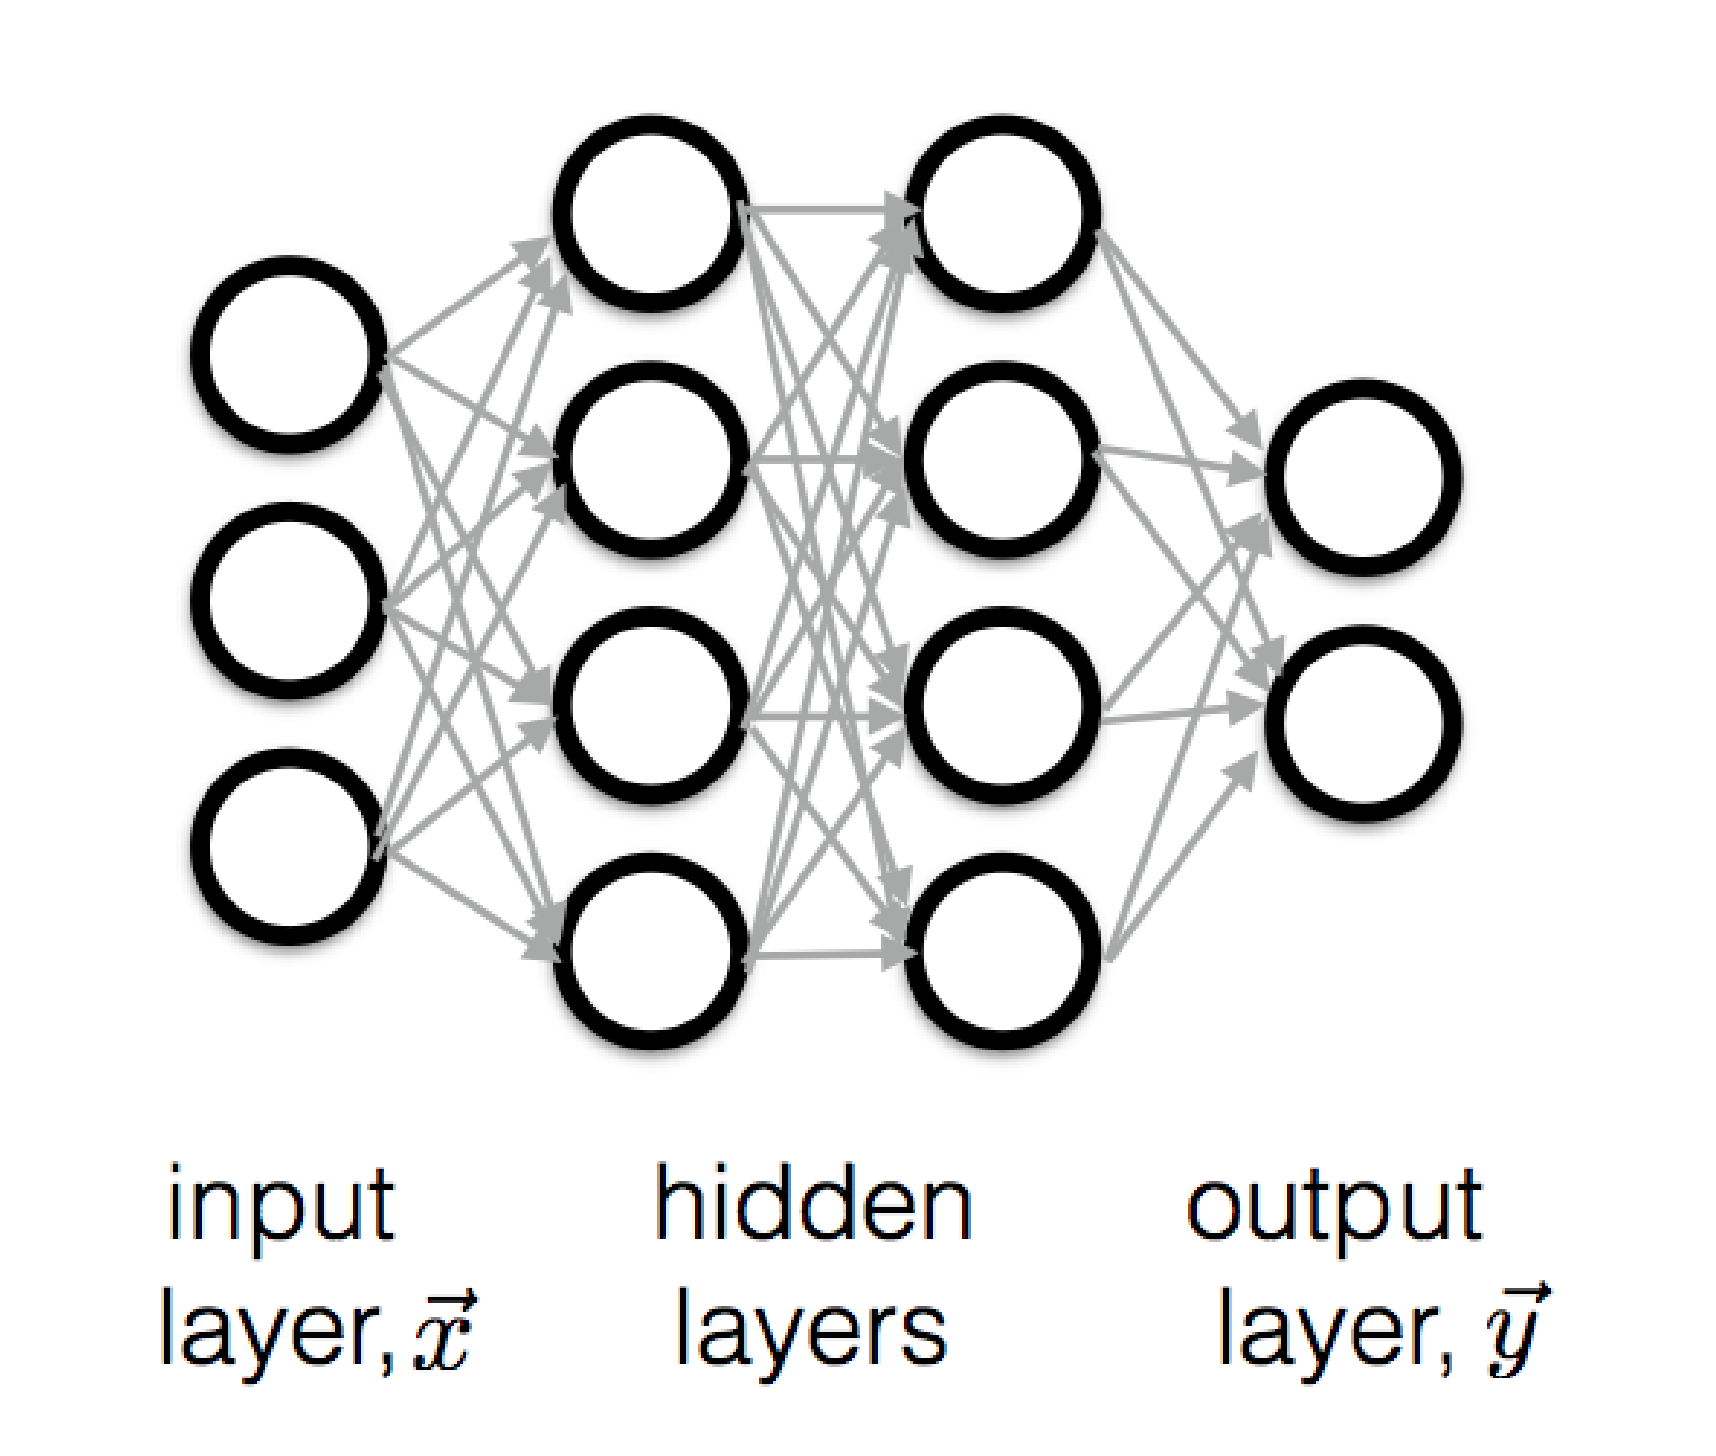
\includegraphics[scale=0.25]{Images/FFNN.png} 
 
 \textbf{Figure 3.} \textit{A graph of a simple FFNN with two hidden layers, that takes in 3 inputs that either classifies into one of two categories or produces two values depending on if the model is completing a classification or regression task. \cite{Acciarri_2}}
\end{figure}

\noindent The algorithm becomes connected network of these weighted sums, where the parameter weights, which are initially random, are learned by giving examples. The network will determine which patterns, or features, correspond to which event, and the algorithm tunes the weights values to produce the desired output through backpropagation. \medskip

\noindent The metric used to determine how effective the model is at the task is the loss function, which is measure of the error between the predicted output and the truth label. For a simple regression task this could be calculated using the mean absolute error or the mean squared error. In the case of particle identification, the problem is one of classification, and the loss function often takes the form of a cross-entropy function, which can be calculated by: 

\[L(y, \hat{y}) = - \sum_{i} y_{i} log(\hat{y}_{i})\]

\noindent where $y$ is the prediction, and $\hat{y}$ is the truth value, over the entire dataset. Here the functions compares the distribution of predictions to the one-hot-encoded true distribution, and the closer the the confidence of that class is to 1, the smaller the loss value. \medskip

\noindent The network looks to minimise the loss by updating the weights and biases of the network with each training step, a process that will fit the network to the data. In order to determine if the loss function is at a minimum, a method of gradient descent is used. The gradient of the loss function is calculated, and the is scaled by a learning rate. A large learning rate will mean that large steps are made, which will reduce the training time, but the optimisation may skip over the minima, while a small learning rate will take longer to converge, but will find the optimal value. Both these methods are subject to finding local minima, rather than the global minima, so stochastic optimiser algorithms are often used to allow for escaping minima, and over time should converge on the correct value. Optimisers often couple these gradient calculations with  variable learning rates, that start of large to allow the algorithm to search the surface, and then reduce in size to allow convergence to take place. \medskip

\noindent In order to prevent the network from continually converging on sub-optimal values, the initial weights are randomly determined. This means that each training process is unique, and the final model will be an ensemble of the models that are produced during each epoch- each pass over the training dataset. The neural networks have a large number of paramaters in order to be able to fit to complex input features, however the model may become too reliant on a small number of weights- which leads to overfitting to the training data, and struggling to generalise to new data. This is an area that will be discussed throughout this report. \medskip

\section{Convolutional Neural Networks}

\noindent In the field of computer vision, the most successful algorithms for pattern detection of images have proved to be Convolutional Neural Networks (CNN). These are ANNs that have been designed to space invariant, which makes them suited to processing images.

\noindent Much like a traditional FFNN, CNNs take in an input, have a number of hidden layers, and return an output; but work differently in that rather than every neuron being connected to each input value, a kernel, a small matrix, is passed over the image, pixel by pixel. This is due to the size of the input which can be several million pixels, where the process would become too computationally expensive to have fully connected layers. This kernel will apply a convolution function, using the pixel and the surrounding pixels as inputs to produce a weighted sum, see Figure 4, which it will produce another image from, with these convolutions detecting local structures \cite{Brenzke} such as edges or other patterns, building several feature maps and through training determining which combinations of these are most important to producing the correct output class, see Figure 5. Each layer passes multiple kernels over the same input, to produce a number of output matrices, all applying a different convolution, to form a tensor as the output.  (In this way, convolutional layers [29] produce many alternative representations of the input image, each serving to extract some feature which is learned from the training sample. \medskip

\begin{figure}[t]
 \centering
 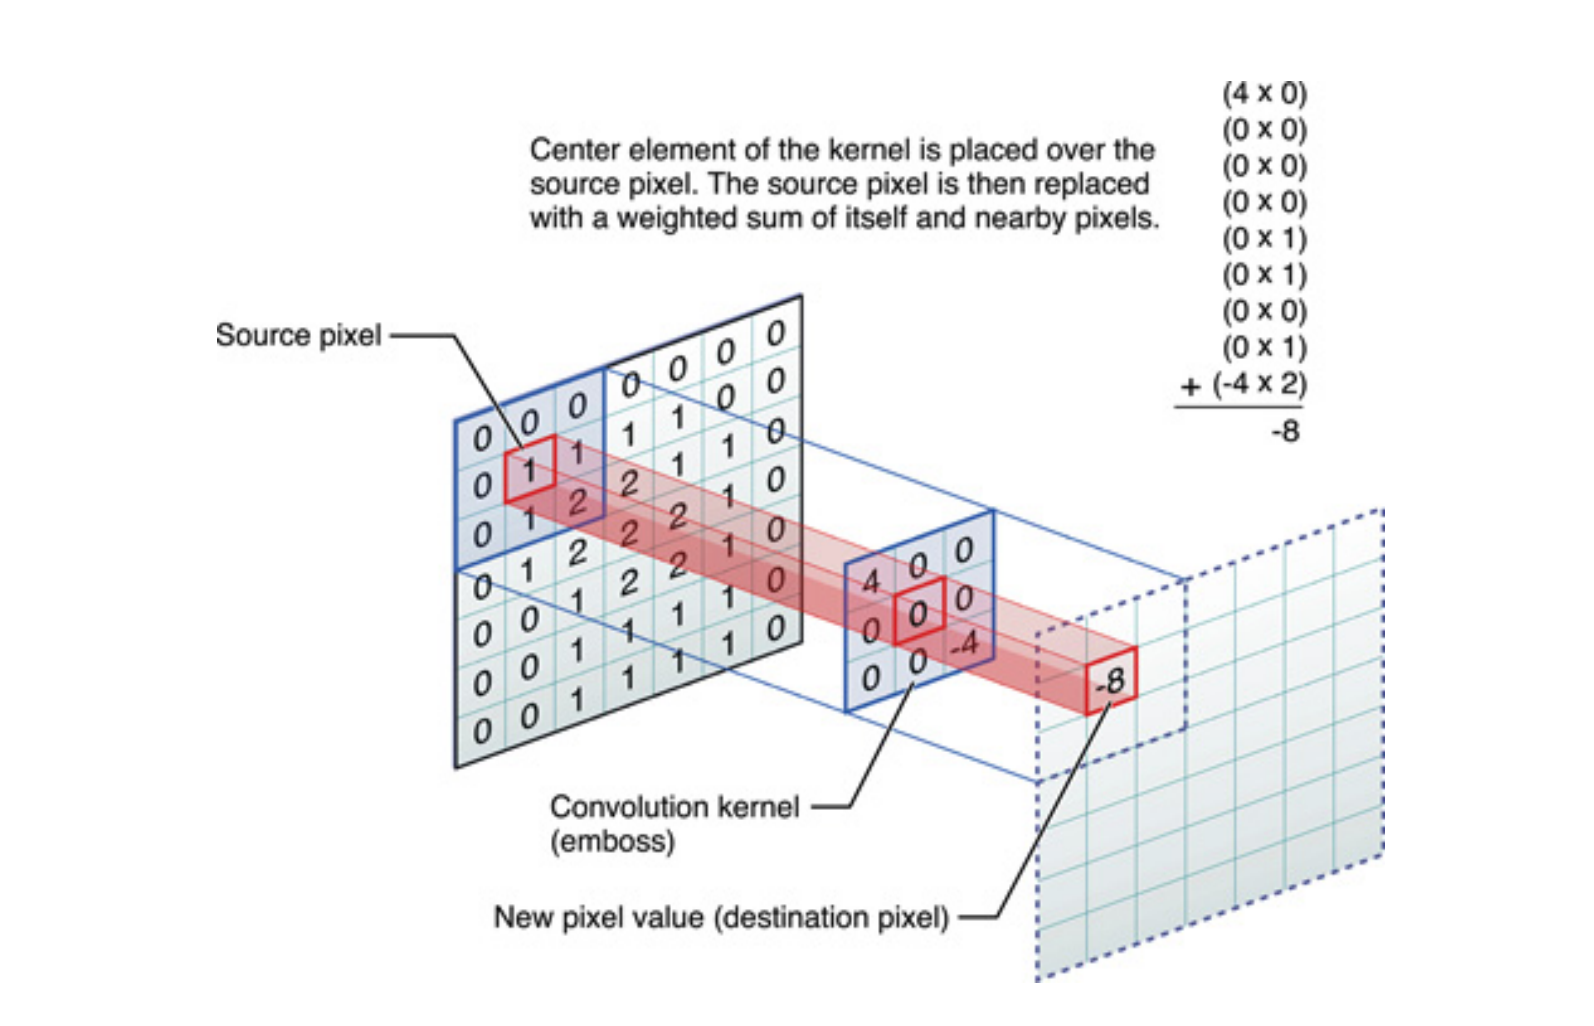
\includegraphics[scale=0.35]{Images/Conv.png} 
 
 \textbf{Figure 4.} \textit{Diagram of a Convolutional Kernel acting on a source matrix. The kernel is placed over a sub grid of the matrix, and the output value is determined by the product of the values in the input grid and the values in the kernel. The kernel then slides across the entire source matrix. \cite{Brenzke}.}
 \end{figure}
 
 \begin{figure}
 \centering
 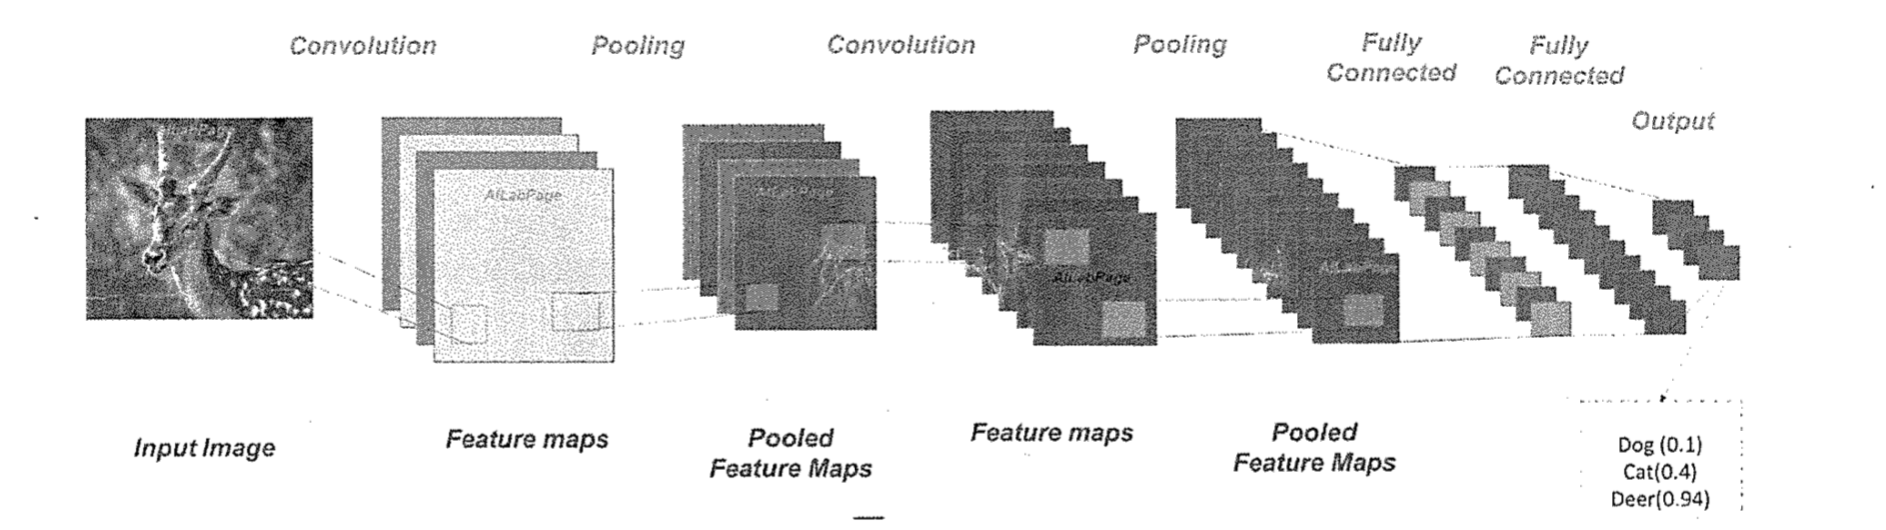
\includegraphics[scale=0.5]{Images/cnn_layers.png} 
 
  \textbf{Figure 5.} \textit{Architecture of a basic CNN, displaying the hidden convolution and pooling layers.}
 \end{figure}

\noindent In order for the network to be able to complete the process in a reasonable amount of time, each convolution layer is followed by a pooling layer, which reduces the size of output feature map by partitioning each matrix into subsections, where either the maximum value of the set (max pooling) or the average of the values (average pooling) is taken, reducing the number of parameters for each subsection to a single value. With these steps of convolutions and pools making up the majority of the layers in the network, producing a final vector, that feeds into a traditional FFNN to produce scores for the confidence level for each label it thinks it may be classifying. It is this output value that cuts are taken on when analysing data, using the simulation results where the score from the network is over a threshold value. \medskip

\section{Robustness}

\noindent A large problem that faces neural networks is the problem of overfitting. This is whereby the model becomes very good at picking up details from the dataset and essentially learns the dataset so much so that it struggles to then generalise on new data. In a CNN as there are fewer free parameters than with a fully connected network then the chance of overfitting is reduced \cite{Brenzke} and methods such as Dropout, which is zeroing random neurons in training so that that the network doesn’t rely on a small number of neurons, can help reduce this. Over a large number of training epochs, the  final network will be ensemble of smaller networks. However, they are still subject to becoming too specialised to the data they have been trained on, and the CNN being used to identify particle events, the model will be trained on the Monte Carlo simulations, neither of which perfectly model real events. This means that the model is susceptible to learning on these unrealistic data sets and becomes inaccurate when fitting for real data. \medskip

\noindent As the two simulations, GibUU differ on how they simulate different interactions, a part of the project was looking at how the models classify events from the two detectors. The robustness of the classifier will be determined by its ability to not show a domain-bias from the generators it was trained on, with the simulations based on models that are not identical to nature.\cite{Perdue} and that the model is able to generalise to incoming detector data. A classifier that is trained to pick up on small details in a dataset, that may be considered noise, will perform poorly on new data that is used in inference, especially if that data is from a different production source, such as a different generator or real detector data. By then poorly classifying incoming data, the experiment loses it's ability to make accurate measurements and identification of the neutrino flavours that are passing through the detector, and as a result loses the ability for accurate oscillation calculations to be made that look at the proportion of neutrinos that change flavour. \medskip

\noindent Many see machine learning algorithms, and in particular deep learning architectures, as black boxes because it is extremely difficult to interpret why they make the decisions they do. As discussed earlier,  the feed forward networks, after training, are a linear combination of the outputs from the nodes in the previous layer, passed through an activation function. Even by looking at the values of these weights and biases, one cannot understand how these values were chosen, and often they are not unique, as training an identical model with identical data will yield a different network, that may produce the same classification output, but have a different set of weights. This is due to the stochastic processes that underpin how the networks are trained, in both the initial weights values before training, and the stochastic processes that determine the loss function backpropagation gradients through the optimiser algorithms such as Adam or Stochastic Gradient Descent \cite{Kingma} . \medskip

\noindent When trying to interpret CNNs the feature maps range from high level features such as edges, to lower more abstract features that would be very difficult for a human to infer meaning from. Research is being undertaken to try and understand these black box algorithms such as \cite{Zhang} which looks at returning a filter over the input image that indicates which parts of the image were the strongest indicators to the network as to why the classification was made. \medskip

\noindent In the case of the particle physics events, the images represent the particle tracks and as a result do not contain as many features themselves as a picture of a object will making the training process for the network more difficult, and the features that the model uses to classify the image potentially more abstract. \medskip

\noindent This problem of interpretability posses a large problem with machine learning algorithms, not because of how they perform, but of whether they can be trusted to make decisions on the part of human experts, whether this being screening for cancers, determining how an autonomous car should act in a critical scenario, or determining whether to approve a mortgage. As a result, it is important that methods are developed to produce understand why these algorithms come to the decisions they do. \medskip

\section{Domain Adversarial Neural Networks}

\noindent An alternative network architecture that will be explored in this project is that of a DANN, which will be joined to the CNN classifier in order to reduce the domain dependence of the model \cite{Bousmalis}. Two sources of data, or domains, are introduced, a source domain where labels are available but not used so that the input is similar to unlabelled data from the target domain where labels are not available. The network produces two classified outputs, a features classifier, which predicts class labels in a way similar to a normal ANN, but also a domain classifier that discriminates between the source and target domains- determining which inputs are from simulations or detector data \cite{Ganin} or in the case of this project determining the inputs from the two different generators, as a proof of concept that in the future these techniques could improve the classification of detector data. \medskip

\noindent DANNs can also be applied to compare multiple simulation only datasets \cite{Perdue}, such as GENIE and GiBUU, to determine whether the network can tell which raw images belong to which. To have a robust model the network will need be invariant to the differences between these, as well as between the simulations and real data. Only data from the source domain is used to determine the parameters for the features classifier, with data from both domains determining those of the domain discriminator. By optimising for accuracy on the features classifier and maximising the error for the domain discriminator the classifier is trained to only use features in both domains. When an equilibrium is reached the domain discriminator is only able to distinguish samples from the sources by chance \cite{Louppe}. Figure 5 shows this additional part of the network, which in theory should produce a network trained to be invariant to the differences in the simulations as well as with real data, and results from \cite{Perdue} at MINERvA showed a small increase in accuracy at ~96\% to ~94.5\% for the domain trained networks.  \medskip

\begin{figure}[b!]
 \centering
 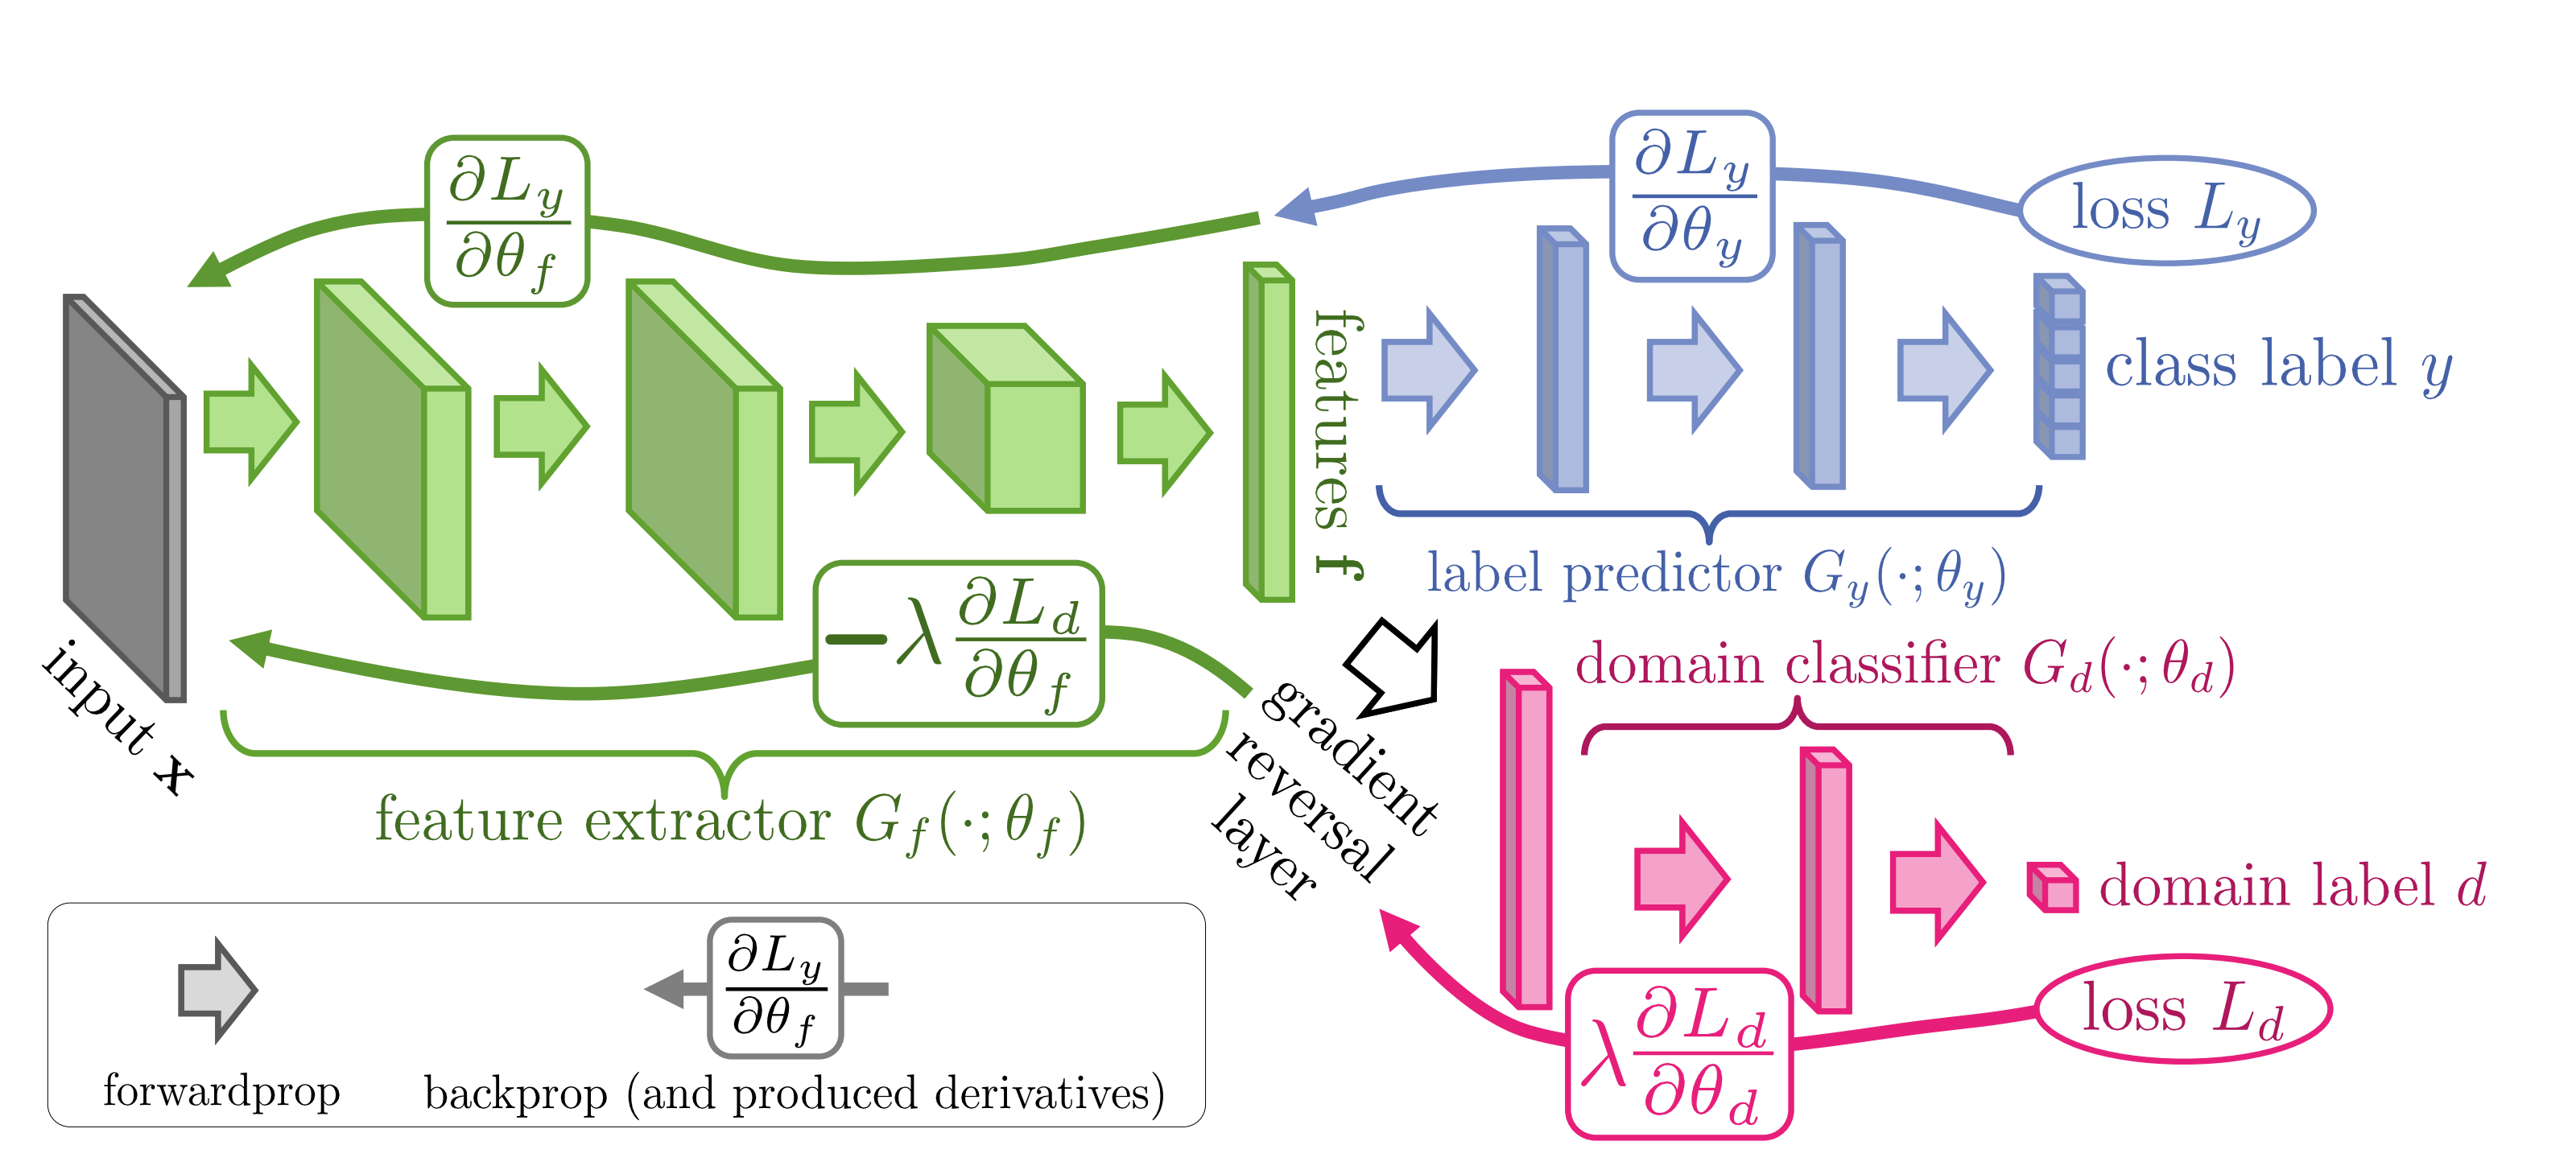
\includegraphics[scale=0.3]{Images/Dann.png} 
 
  \textbf{Figure 6.} \textit{Plot of the architecture of a DANN joined to a network, where $y$ is the outputs from the feature classifier and $d$ the  outputs of the domain classifier. The gradients show the error, or loss, functions that back-propogate to determine the weights and biases. \cite{Ganin}}
\end{figure}